% Target: 4-6 blz

\todo{Meer bronnen?}

Modern web browsers are complex applications consisting of many components that have to work together. To develop a generic algorithm it is crucial to have first an in-depth insight in the working of the engines used to drive a web browser. In this project is foccused on Internet Explorer, Mozilla Firefox, Chromium and Apple Safari. Those four browsers combined have a marketshare of more then 90\%\footnote{http://gs.statcounter.com/\#desktop-browser-ww-monthly-201412-201412-bar} \footnote{http://www.netmarketshare.com/browser-market-share.aspx?qprid=1\&qpcustomb=0}.

All modern web browsers allow the usage of multiple tabs with web pages in a single window. The underlying implementations differ creatly. In some browsers are only libraries provided by the operating system used while others decided to use their own. Also have some vendors decided to use multiple processes, sometimes even a new process for every single tab.

\textbf{Internet Explorer} is the well-known web browser from Microsoft. While until quite some time ago also a Mac version was available, in the last decade only the Windows version has been updated. Since version 7 is tabbed browsing available and version 8 was improved with the abilty to run tabs from their own process (see figure \ref{fig:ie8proc}). This feature is called Loosely-Coupled IE\cite{http://blogs.msdn.com/b/ie/archive/2008/03/11/ie8-and-loosely-coupled-ie-lcie.aspx}. Every process runs independent from the other processes and runs its own network stack and instances of content plugins like Flash or Silverlight.

Starting each tab in its own process comes with an inevitable overhead by using more memory and the time it cost to start the process. For this reason can a process host multiple tabs. The amount of tabs to host in a single process and the maximum of processes to use is determined by the configuration. For backwards compatibility reasons is also the option provided to disable the usage of multiple processes and host all tabs in a single browser process.

The network stack used in Internet Explorer is provided by the Windows operating system and is called WinINet. This library provides high-level access to functions that allows applications to perform HTTP and FTP requests and utility functions for caching, proxys and security. After setting up the library and initiating and configuring the request, WinINet will perform the necessary steps to execute the request. WinINet depends for this on the Winsock library to setup the required network connections and Schannel to provide transparant support for SSL/TLS connections.

\begin{figure}
    \centering
    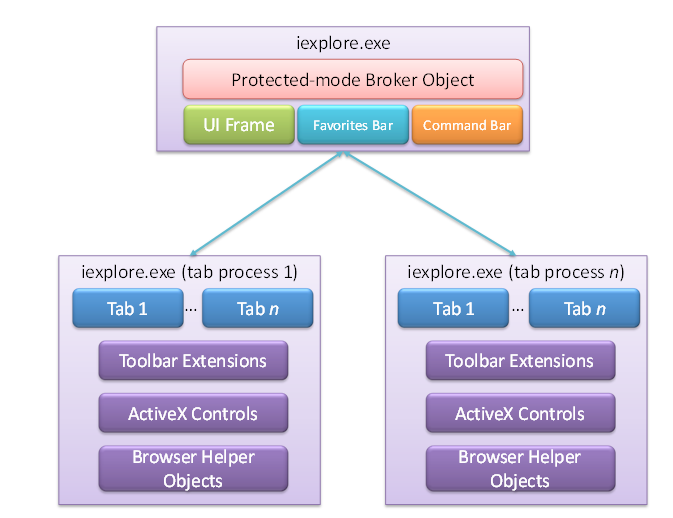
\includegraphics[width=9cm]{Images/IE8_process_model.png}
    \caption{The Internet Explorer process model starting from version 8. \cite{zelfde msdn link, modified}}
    \label{fig:ie8proc}
\end{figure}

\textbf{Firefox} is a cross-platform browser developped by the Mozilla foundation and one of the first that supported tabbed browsing. While it was first the main competitor for Internet Explorer, the release of Google Chrome made it lose some of its popularity.

In Firefox run only the plugins from a different process. The rendering of the web pages still happens from a single process. A longterm project to change that called Electrolysis\footnote{https://wiki.mozilla.org/Electrolysis} has been going on since 2009. In the new architecture is all the rendering moved to a dedicated and sandboxed ``content'' process and is the main process used to host the user interface and serve as a proxy between the outside world and the content process. A longer term goal is to spread the rendering of multiple tabs over more then one content process so that if a content process crashes not all tabs are affected.

To be platform independent is not directly interfaced with the provided libraries of the operating system. Instead a platform-neutral API called NSPR is used. Together with the NSS library that provides the functionality to create SSL/TLS connections is this used by the high-level network library called Necko. Necko provides the interface to perform HTTP and other protocol requests without revealing protocol, transport level or platform specific implementation details and is comparable to WinINet.

\textbf{Chromium} is the open-source version of the Google Chrome browser and are except a couple of proprietary components identical. While it's relative young, it is one of the most used web browsers. The big innovation of Chrome \cite{http://blog.chromium.org/2008/09/multi-process-architecture.html} was to use multiple processes instead of a single process. Besides its own process for every tab, have also the plugins and audio subsystem their own process. The subprocesses run in a sandbox with limited privileges and use the main process to communicate with the outside world.

\begin{figure}[h]
    \centering
    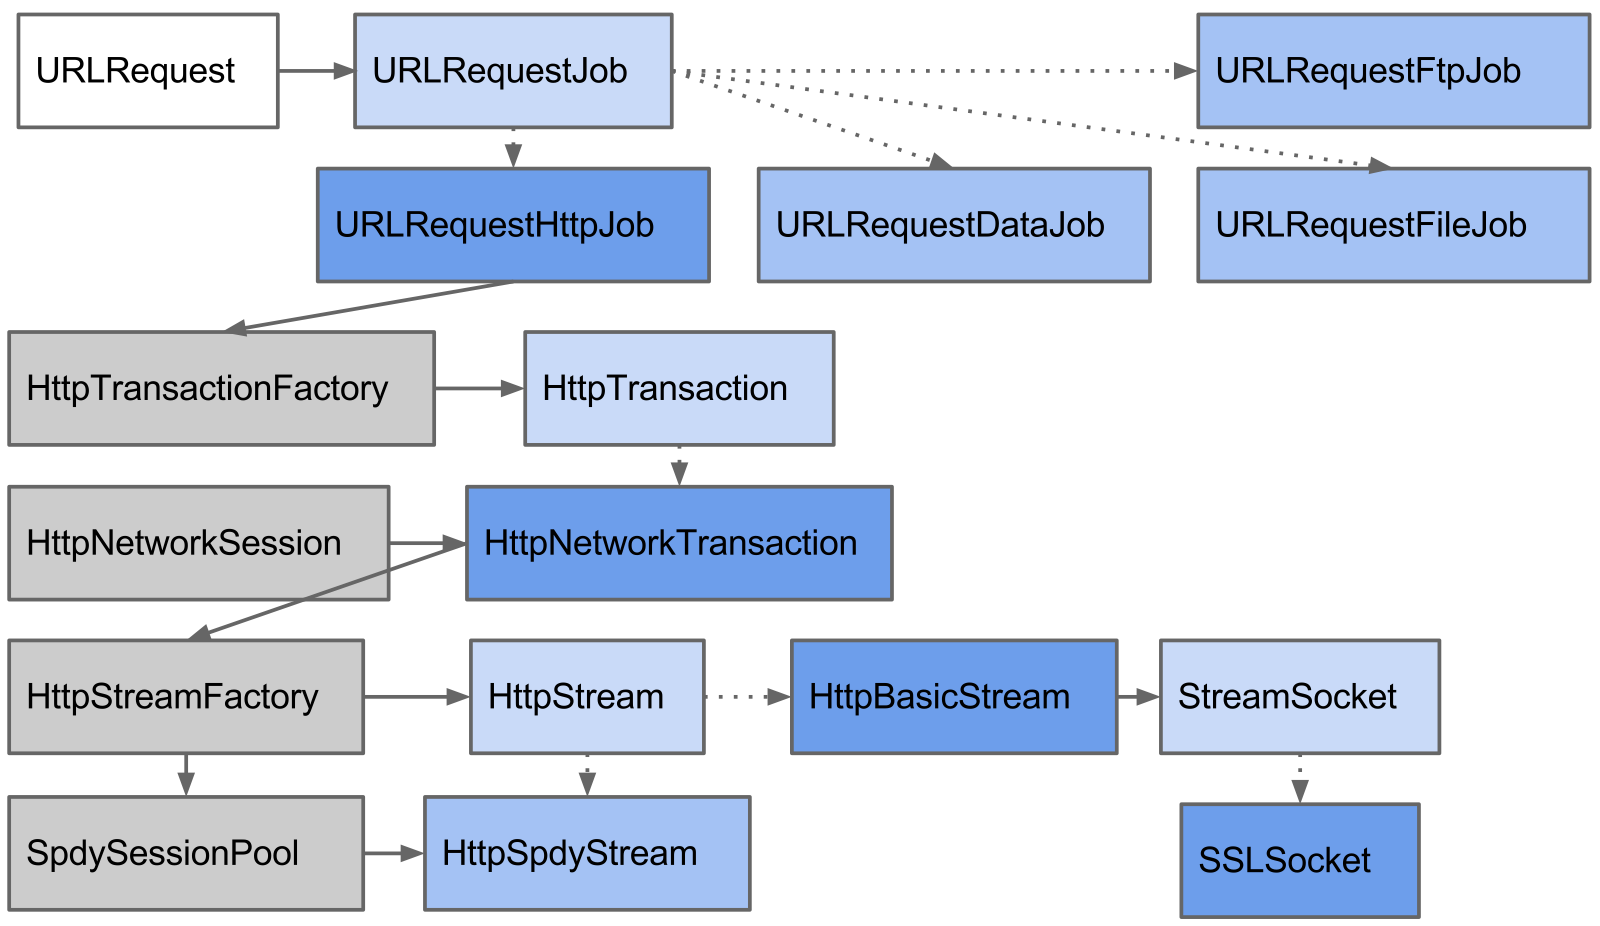
\includegraphics[width=9cm]{Images/Chrome_network.png}
    \caption{A high-level overview of the components involved in requesting an URL in Chromium. Platform specifics details related to sockets are hidden in StreamSocket and the usage of SSL/TLS is made transparant by using the interface-compatible SSLSocket instead of StreamSocket. \cite{http://www.chromium.org/developers/design-documents/network-stack, modified}}
    \label{fig:chrome_network}
\end{figure}

The library used by Chromium for network access is custom developped and tightly integrated in the engine. It provides similary to Necko and WinINet a high-level interface (see figure \ref{fig:chrome_network}) but also it does contain lower level interfaces that interface directly with the operating system socket API. To provide transparant SSL/TLS support is the same library used as in Firefox, NSS.

\textbf{Safari} is the last browser that was examined in this project. It's the proprietary web browser of Apple that is since three years only available for their own operating system, Mac OS X. Around the same time\footnote{https://lists.webkit.org/pipermail/webkit-help/2011-July/002298.html} has support for using multiple processes been added. Safari is closed-source but build on top of many open-source components like JavaScriptCore and WebKit.

Safari uses until a certain limit a dedicated process for every tab. However for performance reasons and resource restrictions is after reaching the limit multiple tabs hosted in a single process. The network operations for the main and tab processes is concentrated in a dedicated process. Only this process will retreive the webpages and use IPC mechanics to deliver the result to the correct process. 

CFNetwork is the library that is used by Safari for its network access. This library is one of the core frameworks of the OS X operating system and available for all applications. It provides interfaces for all relevant web related protocol. An unified interface called NSUrl like the other browsers use is also available, however because of the closed-source nature of Safari it's not possible without an extensive reverse engineering effort to determine if it's used instead of directly using the provided APIs of the CFNetwork library.

\iffalse

Which techniques are used by browsers to make concurrently visiting multiple
URLs possible?
	- Tabs of course
		- As a process
		- As multiple threads under the browser process

How can we link an HTTP request to its source URL without the modification of the used web browser?
we need extra information, see vraag 4
network is niet genoeg blablabla

How do web browsers make HTTP requests and retrieve webpages? Which Operating System level APIs are used?
	- Safari: CFNetwork and NSURLConnection(Loader) and IPC
		1 hoofdprocess: Safari
		1 process per tab: Safari Web Content
		1 process voor networking: Safari Networking
		Network stack of OS X.
	- Internet Explorer: C API calls naar Windows libraries
		Process per tab: is configureerbaar in settings/registry, je kan ook meerdere tabs in 1 process hebben
		Network stack of Windows
	- Firefox: C++ Library calls
		Single Process (+ 1 process voor flash)
		Own network stack Necko (nss3 voor trafiek te encrypten)
		\url{https://developer.mozilla.org/en-US/Firefox/Releases/3.5/Updating_extensions#Getting_a_load_context_from_a_request}
		http://stackoverflow.com/questions/10719606/is-it-possible-to-know-the-target-domwindow-for-an-httprequest
	- Chrome: IPC 
		1 hoofdprocess: Google Chrome die networking doet
		1 process per tab. (Altijd 13 threads?)
		1 process voor Flash.
		1 process voor Audio. (4 threads)
		Own network stack (nss3 voor trafiek te encrypten)
		http://www.chromium.org/developers/design-documents/network-stack

What extra information from the client's (running) machine can be used to augment the information gained from network trac to make the tracking of malware to its source URL easier?  
	- The Thread ID or Process ID van tabs, PDF reader, Java applet, ...
	- Handle bij IE
	- File descriptors
	- Process tree
	- Voordeel van op machine network traffic te intercepten is dat we rommel van andere applicaties niet zien, maar enkel het trafiek van de browser en de gespawnde subprocessen ervan.
	- 
\fi